\subsection{Approach Overview}
\label{sec:overview}

\begin{figure*}[t]
 \centering
 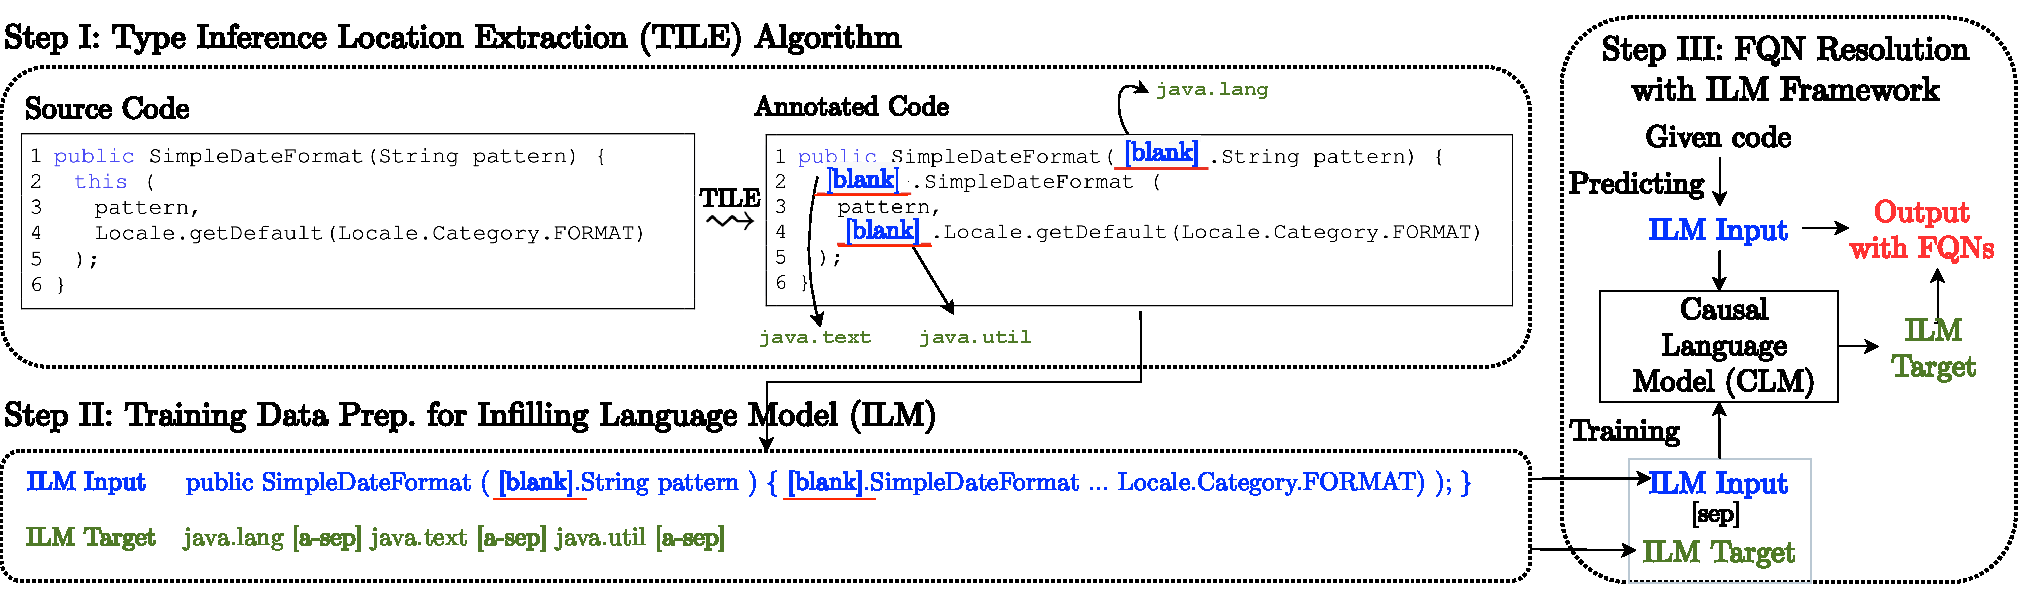
\includegraphics[width=.98\textwidth]{overview-ilm-3.pdf}
 \vspace{-12pt}
 \caption{A general overview of \tool approach for resolving fully-qualified names.}
 \label{fig:approach}
\end{figure*}

%Fig.~\ref{fig:approach} illustrates the general overview of {\tool}. It has two primary components, the first of which is the {\em Type Inference Location Extraction} (TILE) algorithm. Given a code snippet, TILE analyzes it to identify all locations where an API name needs to be expanded. Next, at each of these type inference locations, it inserts a \blank token to represent the missing part of the fully-qualified name (FQN). Let us refer to the resulting \blank inserted code snippet as \blank-code.

Fig.~\ref{fig:approach} illustrates the general overview of
{\tool}. It has two primary components, the first of which is the {\em
  Type Inference Location Extraction} (TILE) algorithm (Step I). Given
a code snippet, TILE analyzes it to identify all the code locations
where an API name needs to be expanded. Next, at each of these type
inference locations, it inserts a \blank token to represent
the missing part of the fully-qualified name (FQN). Let us refer to
the resulting \blank inserted code snippet as
\blank-code. This step is applied during both training and
inference. However, during training, successfully compiled source code is 
utilized due to which all the FQNs of the API elements are resolved. 
%That is, all the blanks have the corresponding FQNs. Thus, in training, the
%\blank-code with the respective FQNs is referred to as
%annotated code.
Thus, all the blanks have one-to-one correspondence with their
FQNs. We refer to this combination of the \blank-code with their FQNs
as the {\em annotated code}.

%The goal of the next stage is to infer all FQNs corresponding to the \blank tokens in the \blank-code. As discussed in Section~\ref{sec:key}, an effective FQN resolution solution incorporates the inter-connections between API and program elements. Thus, we consider the Infilling Language Model (ILM) introduced by Donahue et al.~\cite{} as the next component in our approach. Unlike standard language models (LMs), the ILM framework is capable of incorporating context on both sides of the blank, which in turn facilitates inter-API dependency learning. Such contextual knowledge coupled with ILM's ability to effectively predict missing spans of text helps \tool derive FQNs at all relevant API locations.

The goal of FQN resolution is to infer all FQNs corresponding to the
\blank tokens in the \blank-code. As discussed in
Section~\ref{sec:key}, an effective FQN resolution solution
incorporates the inter-connections between API and program
elements. Thus, we consider the Infilling Language Model (ILM)
introduced by Donahue {\em et al.}~\cite{donahue-etal-2020-enabling} as the next component in
our approach. 
%The actual neural network model is called Causal
%Language Model (CLM).
Behind the scenes, the ILM framework utilizes a Causal Language Model (CLM).
% Unlike standard language models (LMs), the ILM
% framework is capable of incorporating context on both sides of the
% blank, which in turn facilitates inter-API dependency learning. 
However, it recasts the input with a pre-specified set of keywords to
enable it to incorporate context on both sides of the blank, which in
turn {\em facilitates inter-dependency learning among API elements}.
Such contextual knowledge coupled with ILM's ability to effectively
predict missing spans of text helps \tool derive FQNs at all the API
locations at once.

For training the model (Step II), the annotated code is 
used in which the \blank-code serves as the ILM input, and the prefixes
of the corresponding FQNs serve as the ILM target.

For FQN resolution (Step III), the given code without FQNs is first analyzed
by TILE to produce the ILM input. 
%The trained ILM model will produce the ILM target, which contains all the FQNs corresponding to the blanks in the ILM input. 
From the ILM input, the trained CLM model within the ILM framework predicts the ILM target, which essentially contains all the FQNs corresponding to each of the \blank tokens in the input.
Finally, combining the ILM input and the
ILM target, we can obtain the 
%final code with the FQNs of the API elements.
FQN-annotated version of the given code snippet.



%%%\begin{figure}[t] %[!htp]
%%%	\centering
%%%	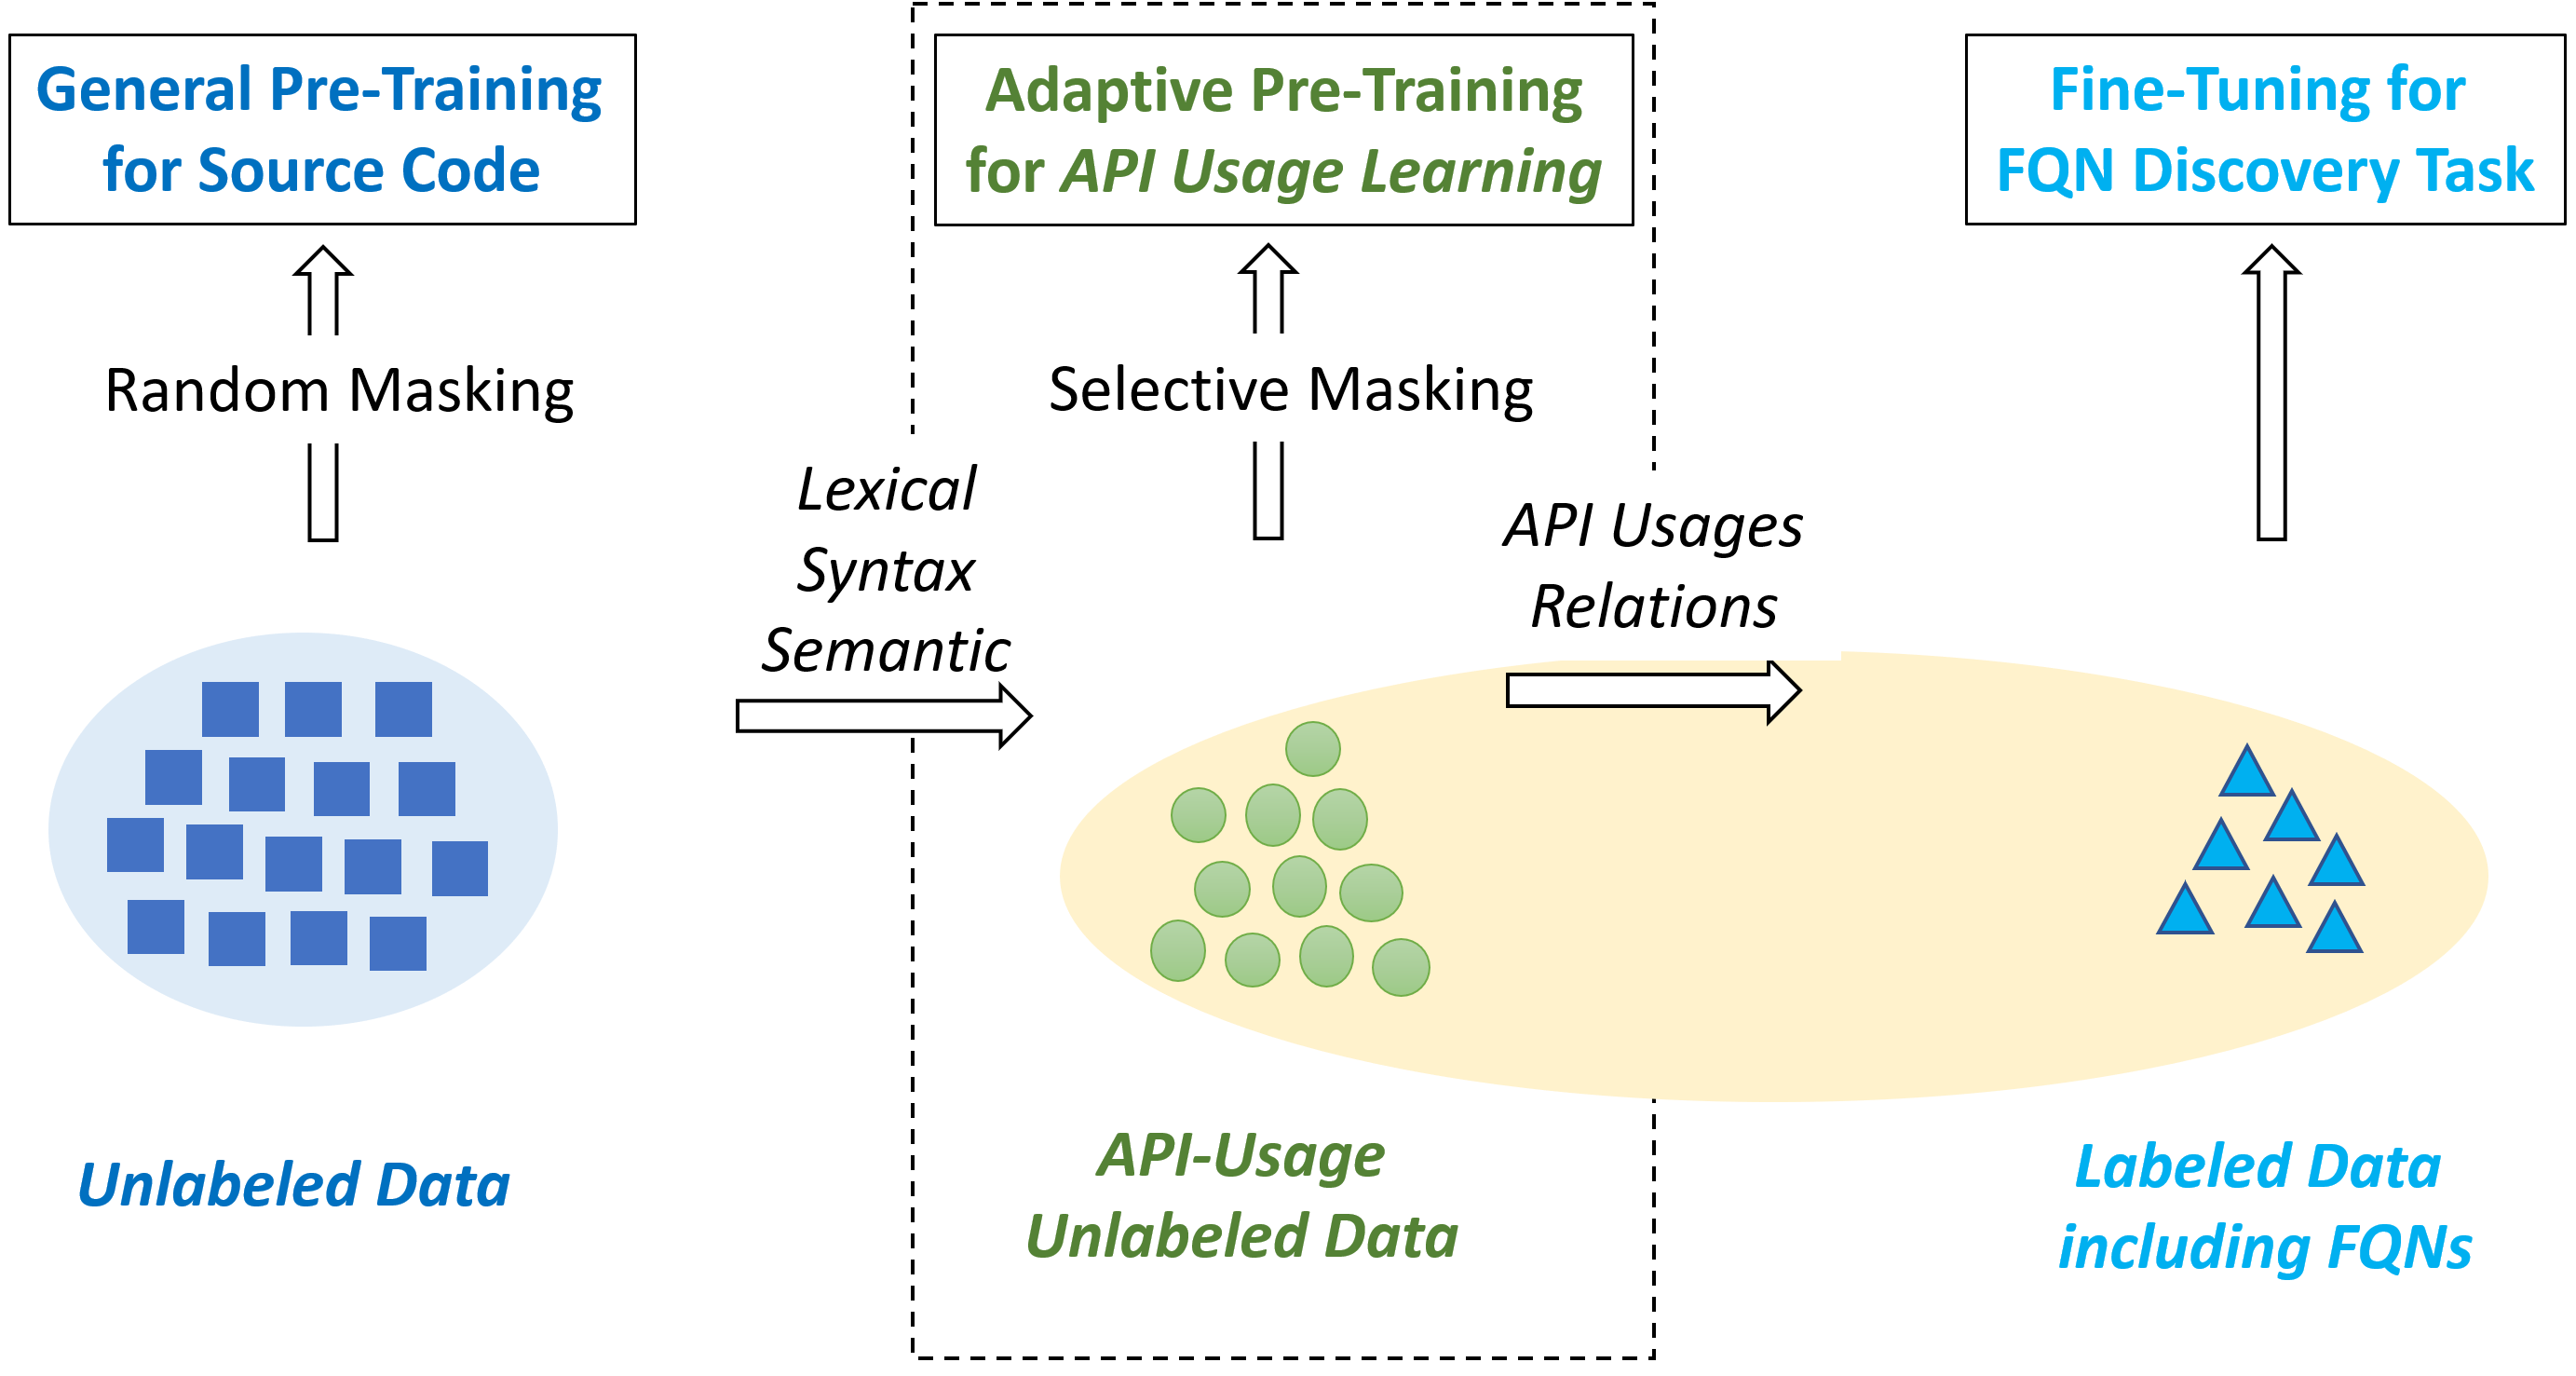
\includegraphics[width=\linewidth]{overview}
%%%        \vspace{-12pt}
%%%	\caption{{\tool} Overview with FQN-Guided Pre-Training}
%%%	\label{fig:overview}
%%%\end{figure}
%%%
%%%Figure~\ref{fig:overview} shows {\tool}'s overview. The
%%%state-of-the-art approaches in using pre-training language models
%%%often follow the pre-train-then-fine-tuning paradigm. The pre-training
%%%is task-agnostic and the fine-tuning usually suffers from the
%%%insufficient supervised training data. In {\tool}, inspiring by Gu
%%%{\em et al.}~\cite{gu-emnlp20}, we use a three-stage solution with the
%%%addition of the task-guided pre-training stage. We dedicate the
%%%task-guided pre-training stage {\em to learning API usage patterns} to
%%%help with the fully-qualified name detection task.
%%%
%%%The first stage is dedicated to the general pre-training on source
%%%code to help {\tool} learn the general lexical, syntax, and semantic
%%%characteristics of source code. For this purpose, we use
%%%CodeBERT~\cite{codebert} in which we randomly mask 15\% tokens and
%%%train the model to reconstruct the original code tokens.
%%%
%%%The second stage is aimed to effectively and efficiently learn the
%%%{\em API usage patterns} and {\em the dependencies among API elements
%%%  and the relevant program elements} in source code. From the source
%%%code without any labels (unlabeled data), we apply a selective masking
%%%strategy to focus on masking the important tokens for the FQN
%%%discovery task. From the motivation and key ideas, we identify as
%%%important the tokens corresponding to the API elements and relevant
%%%program entities via the API usage relations/dependencies. Note that
%%%the training data at this stage unlabeled as in the general
%%%pre-training stage. We expect that the model will learn the API usage
%%%patterns and relations among the code elements that complement to the
%%%general knowledge learned from the general pre-training stage. The
%%%details on our selective masking are presented later.
%%%
%%%The fine-tuning stage is dedicated to the task of recovering the FQNs
%%%in source code. It will be trained with the labeled data, i.e., with
%%%the FQNs. We can obtain such labeled data by running a program
%%%analysis tool or a compiler on a complete code.

%with the masking process that emphasizes on learning API usages and
%patterns with the unsupervised data on the dependencies/relations
%among API elements and relevant program elements.

